% Hopefully this will be the final version of Problem statement.
\section{Problem Statement}

Cloud providers spend huge amount of money on data centers because a typical data center consumes as much energy as 25,000 households \cite{Dayarathna:2016ua}. Thus, reducing the energy consumption becomes the major concern of Cloud providers. 
In addition, data centers and computation powers are the pillars of modern Cloud computing industry, software industry and etc. Reducing the cost of data centers will lead to a reduction of cost of softwares which consequently be beneficial to most people who access the Internet on a daily basis.
Among several components that consume energy such as cooling system, physical machines (PMs) (e.g servers), and network devices, PMs accounts for 40\% and have a huge improvement space, since they always run in a low utilization (e.g from 10\% to 50\% of required resources on average) \cite{Barroso:2007jt,Shen:2015hm}. This low utilization of resource problem can be solved by fine granularity management of Cloud resources (e.g CPUs and RAMs) using a new virtualization technology: containers \cite{Felter:2015ki, Soltesz:2007cu} and a new service model: Container as a Service (CaaS) \cite{Piraghaj:2015uf}. Container is an operating system (OS) level of virtualization which means multiple containers  run on a VM and share the OS. CaaS uses containers as the fundamental resource management units.  That is, instead of deploying applications on VMs, applications are now deployed in containers which are running on top of VMs. In terms of Cloud resource allocation, the advent of container makes it possible to improve the utilization inside VMs, and consequently, achieve more reduction of energy consumption. 
% is a mixture of traditional IaaS (Infrastructure as a Service) \cite{Mell:2011jj} and PaaS (Platform as a Service); it 


\begin{figure}
	\centering
	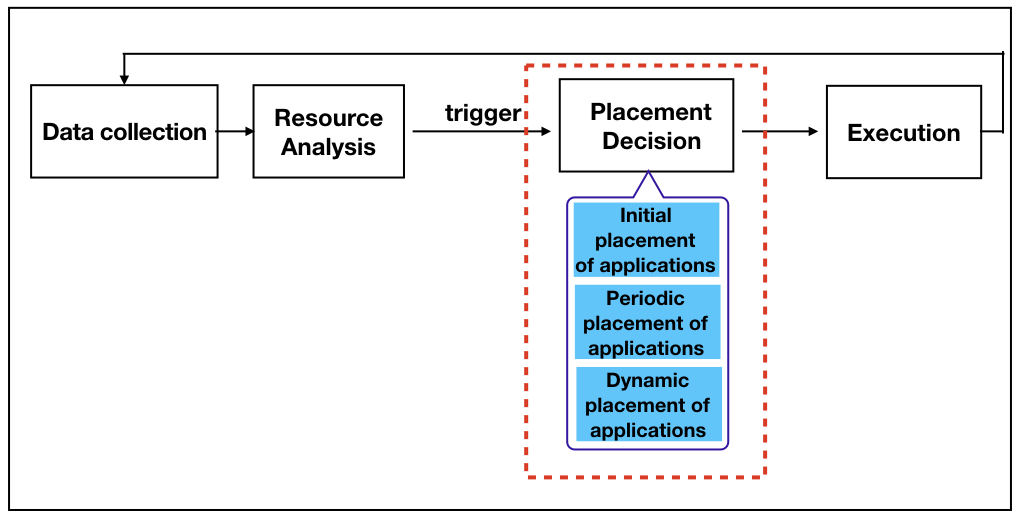
\includegraphics[width=0.7\textwidth]{pics/workflow_management.png}
	\caption{A workflow of resource management \cite{Mishra:2012kx}}
	\label{fig:workflow}
\end{figure}

Server consolidation \cite{Varasteh:2015fu} is the core strategy in improving the utilization throughout the Cloud resource management processes as shown in Figure \ref{fig:workflow}. Three management processes: new application allocation \cite{Jennings:2015ht}, periodic optimization \cite{Mishra:2012kx}, overloading and under-loading adjustments \cite{Mishra:2012kx} have distinct characteristics, hence, the server consolidation techniques applied on them can be roughly classified into two categories: static \cite{Xiao:2015ik} and dynamic \cite{Beloglazov:2012bw}.
Static approaches use estimated resource utilization of applications (e.g average resource utilization of historical data) as the input to combine applications to a minimum number of PMs \cite{Mishra:2012kx}. Static consolidation normally involves large amount of applications and PMs, therefore, the optimization is quite time-consuming and often conducted in a proactive (Cloud providers initiate.) and off-line fashion. Periodic optimization belongs to this category. It takes a number of existing applications and re-allocate them into a number of PMs. 

Static server consolidation are detailed explained in terms of VM-based and container-based Cloud. In a traditional VM-based Cloud, server consolidation can be described as, given a number of  PMs which can be represented as resources (e.g CPU cores and RAM etc); a number of requests for fixed configurations of VMs (assume applications have been deployed in VMs), the configuration can also be represented as aforementioned resources; The objective is to allocate these requested VMs into a minimum number of PMs. The decision variable is the location of each requested VM. The basic constraint is that the aggregative resources  of hosted VMs cannot exceed the PM's resource capacity. 

In contrast, in a container-based Cloud, instead of allocating requested VMs in PMs, a set of containers (assume applications have been deployed into containers) represented as resources is first allocated to a number of fixed type VMs, then, these VMs are allocated to PMs. The decision variables are the allocation of containers (upper level) to VMs and the allocation of VMs (lower level) to PMs. For the upper level of allocation, the objective is to maximize the utilization of resources (e.g a balanced utilization among several resources), while the lower level objective is to minimize the number of PMs. The constraint is the demand of containers not to exceed the VM's capacity and the demand of hosted VMs not to exceed the PM's resource capacity. An additional constraint is that each container has its OS requirement which makes them cannot be simply packed into homogeneous VMs. 

Dynamic approaches take one application each time, allocates it into one of the PMs \cite{Xiao:2015ik}. The operation is conducted in an online fashion, therefore, it requires fast reaction. Overloading and under-loading can be categories to dynamic consolidation problem \cite{Beloglazov:2013ht}.  
In VM-based Cloud, the dynamic problem can be described as given a set of VMs and PMs, allocate these VMs to PMs iteratively so that the final solution reaches a global optimal state.
The key point is that the migration of VM can be conducted immediately after its position is decided. Hence, essentially, the problem can be simplified to allocating one VM to PMs. The difficulty is that the iterative process is hard to reach a global optimal because it normally follows a greedy-based approach such as First Fit. In container-based Cloud,  the problem is even complicated, if no VM can accommodate a container, a new VM must be created, which incurs a second level of deployment.

New application allocation can be seen as either static: allocate a batch of new applications, or dynamic: allocate a new application each time. In this proposal, we consider it in both ways.

Traditional VM-based server consolidation are modeled as bin-packing problems \cite{Mann:2015ua}. This is because VMs and PMs are naturally modeled as items and bins and server consolidation and bin-packing have the same optimization objective: minimize the number of bins/PMs as the number of PM is proportional to the energy consumption. The complexity of bin-packing problem is NP-hard which means it is extreme time-consuming to find its optimal solution when the number of decision variables is large. Container-based server consolidation can be categorized as a bilevel optimization problem \cite{Colson:2007bu}. Bilevel problems are typically non-convex and strongly NP-hard \cite{Vicente:1994ie}. In this case, two levels are lower-level: Containers to VM and upper-level: VMs to PMs. These two levels optimization are connected through decision variables. In this case, two levels of optimization are both bin packing problems and they are cooperating \cite{Legillon:2012dd}.

Currently, most research focus on VM-based server consolidation and these methods can not be directly applied on container-based consolidation because of the different structure. Only few research focus on container-based server consolidation problem. One of the state-of-the-art research is from Piraghaj and et al \cite{Piraghaj:2015uf}. They first propose a VM-resizing technique that defines the types of VM based on analyzing the historical data from Google. Then they propose a two-step allocation: first allocate containers to VMs and then allocate VMs to PMs. Their major contribution is the method of defining types of VM. The allocation of containers does not optimize the energy consumption and the allocation of VMs are traditional First Fit algorithm. In addition, they propose a dynamic consolidation \cite{Piraghaj:2016bw} using a series simple heuristics such as Random Host Selection Algorithm or First Fit Host Selection. 
Their resource allocation system completely relies on dynamic consolidation without using static methods. Although their system can execute allocation fast, the energy efficiency cannot be guaranteed.
The reasons are mainly from two aspects, firstly, they mainly rely on simple bin-packing algorithms to allocate containers to VMs. As Mann's research \cite{Mann:2015ua} showed, server consolidation is a lot harder than bin-packing problem because of the multi-dimensional of resources, heterogeneous PMs, migration cost etc. Therefore, general bin-packing algorithms do not perform well. Secondly, they use a two-step allocation. Because of the interaction of two allocations, separated optimization approach will lead to local optima \cite{Mann:2016hx}. Therefore, these two allocations should be considered simultaneously.

The overall goal of this thesis is to develop new container-based server consolidation approaches to solve three problems: joint allocation of containers  and VMs, periodic global optimization and dynamic consolidation. 
